\section{Tiền xử lý và Tích hợp dữ liệu (ETL Pipeline)}

\subsection{Kiến trúc Tổng quan Hệ thống ETL}

Quá trình tiền xử lý, chuẩn hóa và tích hợp dữ liệu từ các nguồn phân tán được tự động hóa hoàn toàn thông qua nền tảng \textbf{Pentaho Data Integration (PDI / Spoon)}. Kiến trúc luồng dữ liệu được thiết kế chặt chẽ theo mô hình 3 lớp tiêu chuẩn nhằm tối ưu hóa hiệu năng, bảo đảm tính toàn vẹn và khả năng mở rộng của hệ thống:
\begin{enumerate}
    \item \textbf{Vùng tiếp nhận (Landing Zone - định dạng CSV):} Điểm tập kết ban đầu của các tệp dữ liệu thô nguyên bản (RAW CSV) trích xuất từ các bộ dữ liệu gốc, đồng thời liên tục tiếp nhận các gói dữ liệu mới khai thác (crawled data) từ luồng luân chuyển của Steam Crawler. Dữ liệu thô luân chuyển được tổ chức phân vùng thư mục hạ tầng theo cú pháp \texttt{Datasets/landing/extract\_dt=YYYYMMDD/} chứa các tệp trọng tâm như \texttt{players.csv}, \texttt{history.csv}, \texttt{reviews.csv}, \texttt{purchased\_games.csv}, \texttt{private\_steamids.csv}, \texttt{achievements.csv}, và \texttt{games.csv}.
    \item \textbf{Vùng đệm tiền xử lý (Staging Area - MSSQL):} Đóng vai trò là phân vùng đệm trung gian chứa dữ liệu tạm thời, cô lập luồng dữ liệu thô trước khi can thiệp sâu. Vùng Staging được thiết lập cơ chế tự động làm sạch triệt để sau mỗi chu kỳ nạp dữ liệu thành công, bảo đảm tối ưu hóa tài nguyên lưu trữ và tránh xung đột dữ liệu giữa các phiên làm việc.
    \item \textbf{Kho dữ liệu trung tâm (Data Warehouse - PostgreSQL):} Nơi lưu trữ dữ liệu tập trung đã qua xử lý, làm sạch và chuẩn hóa cấu trúc.
\end{enumerate}

\begin{figure}[H]
    \centering
    \IfFileExists{Images/Pentaho/full_run.png}{
        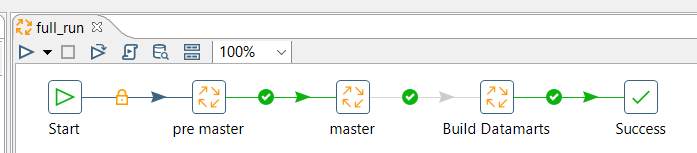
\includegraphics[width=0.9\linewidth]{Images/Pentaho/full_run}
    }{
        \fbox{\begin{minipage}{0.9\linewidth}
            \centering
            \vspace{2cm}
            [IMAGE PLACEHOLDER]\\
            \texttt{Images/Pentaho/full\_run.png}\\
            \vspace{2cm}
        \end{minipage}}
    }
    \caption{Toàn cảnh quá trình thực thi Full Run Pipeline}
    \label{fig:pentaho_full_run}
\end{figure}

Quá trình chạy toàn bộ hệ thống (Full Run) bao gồm hai luồng chính chạy nối tiếp nhau: luồng nạp gốc \textbf{Pre-Master} và luồng tự động hóa \textbf{Master}.

\subsection{Chi tiết Kiến trúc các Luồng Thực thi}

\subsubsection{Luồng Khởi tạo Dữ liệu Lịch sử (Pre-Master)}

\begin{figure}[H]
    \centering
    \IfFileExists{Images/Pentaho/pre_master.png}{
        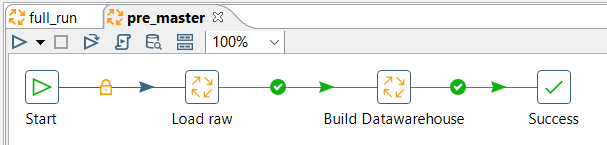
\includegraphics[width=0.7\linewidth]{Images/Pentaho/pre_master}
    }{
        \fbox{\begin{minipage}{0.7\linewidth}
            \centering
            \vspace{2cm}
            [IMAGE PLACEHOLDER]\\
            \texttt{Images/Pentaho/pre\_master.png}\\
            \vspace{2cm}
        \end{minipage}}
    }
    \caption{Luồng Pre-Master nạp dữ liệu gốc ban đầu}
    \label{fig:pentaho_pre_master}
\end{figure}

Luồng \textbf{Pre-Master} chịu trách nhiệm nạp toàn bộ lượng dữ liệu lịch sử khổng lồ từ tập dữ liệu ban đầu. Các bước thực thi bao gồm:
\begin{itemize}
    \item Đọc dữ liệu từ các file RAW CSV gốc.
    \item Nạp dữ liệu vào các bảng trong Staging Area (MSSQL).
    \item Chuyển và xử lý dữ liệu từ Staging Area sang Data Warehouse (PostgreSQL).
\end{itemize}

\subsubsection{Luồng Vận hành và Cập nhật Tự động (Master)}

\begin{figure}[H]
    \centering
    \IfFileExists{Images/Pentaho/master.png}{
        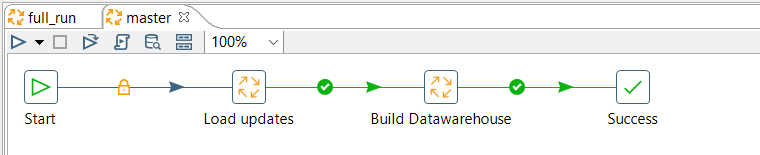
\includegraphics[width=0.9\linewidth]{Images/Pentaho/master}
    }{
        \fbox{\begin{minipage}{0.9\linewidth}
            \centering
            \vspace{2cm}
            [IMAGE PLACEHOLDER]\\
            \texttt{Images/Pentaho/master.png}\\
            \vspace{2cm}
        \end{minipage}}
    }
    \caption{Luồng Master xử lý và cập nhật dữ liệu thu thập mới}
    \label{fig:pentaho_master}
\end{figure}

Luồng \textbf{Master} là luồng được thiết lập để \textbf{lên lịch chạy tự động} trong hệ thống sản xuất. Chức năng chính của Master là:
\begin{itemize}
    \item Quét và xác thực sự hiện diện của dữ liệu mới được thu thập trong thư mục Landing. Quy trình xác thực Landing (Phase 00) được thực thi qua job \texttt{00\_validate\_landing.kjb} kết hợp các transforms rà soát thư mục con phân vùng. Hệ thống đối chiếu chéo với bảng kiểm toán \texttt{dbo.stg\_load\_audit} (nơi \texttt{status = 'success'}) nhằm xác định phân vùng cũ nhất chưa được xử lý, lưu vết đường dẫn vào biến Pentaho đồng thời bỏ qua các phân vùng đã hoàn tất nhằm bảo đảm tính lũy đẳng (idempotency).
    \item Nạp các dữ liệu mới này vào vùng đệm Staging.
    \item Chuyển từ Staging vào Data Warehouse để cập nhật dữ liệu mới nhất.
\end{itemize}

\subsection{Quy trình Tiền xử lý và Làm sạch Dữ liệu Chuyên sâu}

\subsubsection{Giai đoạn Nạp Dữ liệu vào Vùng đệm (Staging Load)}

Dữ liệu thô từ file CSV được đọc và đẩy vào các bảng đệm tạm thời tại MSSQL. Trong quy trình nạp thô (Phase 05 và Phase 10), hệ thống hỗ trợ các luồng chuyển đổi đọc thử nghiệm (optional preview) nhằm kiểm tra cấu trúc tệp (tiêu đề, số lượng cột) mà không thực hiện ghi nhận dữ liệu. Tiếp đó, 5 luồng chuyển đổi song song nạp dữ liệu thô vào các bảng đệm \texttt{dbo.stg\_players}, \texttt{stg\_history}, \texttt{stg\_reviews}, \texttt{stg\_purchased\_games}, và \texttt{stg\_private\_steamids} thuộc cơ sở dữ liệu \texttt{DW\_Staging}. Toàn bộ các trường thông tin tại vùng đệm đều được lưu trữ nguyên bản dưới định dạng chuỗi ký tự động \texttt{NVARCHAR(MAX)} nhằm tránh hao hụt thông tin đầu vào.

\begin{figure}[H]
    \centering
    \IfFileExists{Images/Pentaho/Stage_Raw.png}{
        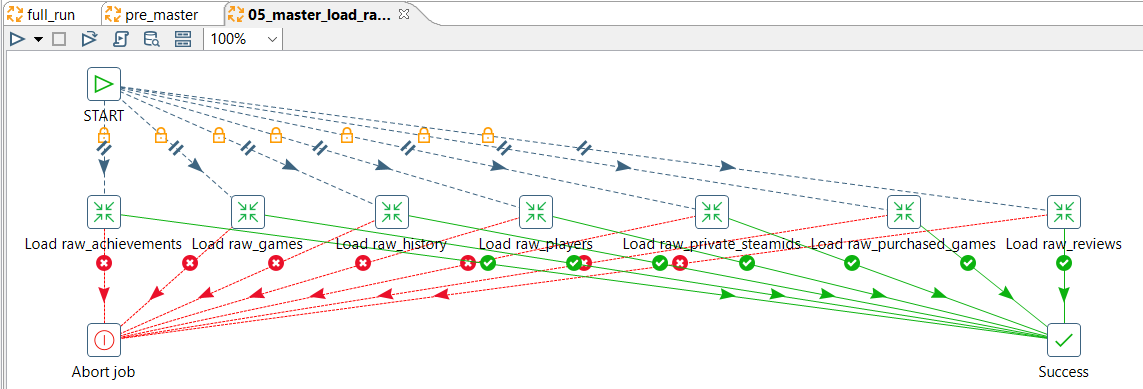
\includegraphics[width=0.7\linewidth]{Images/Pentaho/Stage_Raw}
    }{
        \fbox{\begin{minipage}{0.7\linewidth}
            \centering
            \vspace{2cm}
            [IMAGE PLACEHOLDER]\\
            \texttt{Images/Pentaho/Stage\_Raw.png}\\
            \vspace{2cm}
        \end{minipage}}
    }
    \caption{Quá trình nạp dữ liệu thô vào Staging}
    \label{fig:pentaho_stage_raw}
\end{figure}

\begin{figure}[H]
    \centering
    \IfFileExists{Images/Pentaho/Stage_Update.png}{
        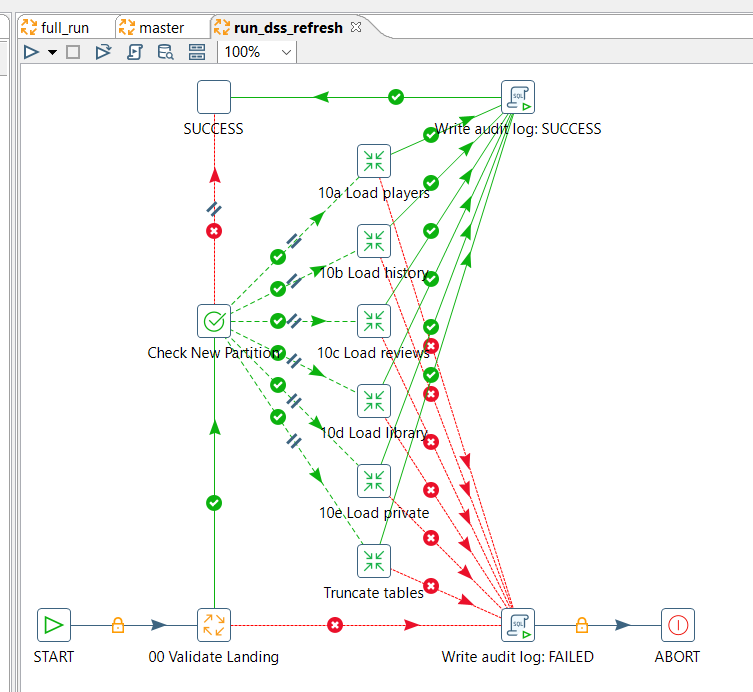
\includegraphics[width=0.7\linewidth]{Images/Pentaho/Stage_Update}
    }{
        \fbox{\begin{minipage}{0.7\linewidth}
            \centering
            \vspace{2cm}
            [IMAGE PLACEHOLDER]\\
            \texttt{Images/Pentaho/Stage\_Update.png}\\
            \vspace{2cm}
        \end{minipage}}
    }
    \caption{Quá trình nạp dữ liệu cập nhật vào Staging}
    \label{fig:pentaho_stage_update}
\end{figure}

\subsubsection{Giai đoạn Xây dựng Data Warehouse (Build DW)}

Đây là bước thực hiện các thao tác tiền xử lý dữ liệu của toàn bộ pipeline ETL.

\begin{figure}[H]
    \centering
    \IfFileExists{Images/Pentaho/Build_DW.png}{
        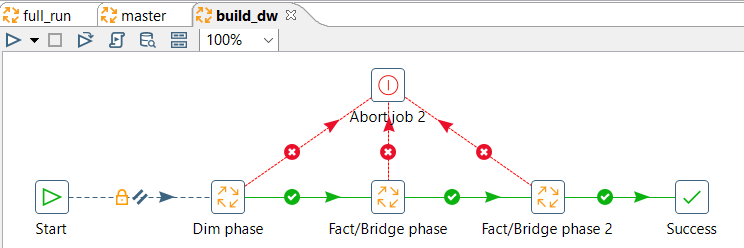
\includegraphics[width=0.7\linewidth]{Images/Pentaho/Build_DW}
    }{
        \fbox{\begin{minipage}{0.7\linewidth}
            \centering
            \vspace{2cm}
            [IMAGE PLACEHOLDER]\\
            \texttt{Images/Pentaho/Build\_DW.png}\\
            \vspace{2cm}
        \end{minipage}}
    }
    \caption{Quá trình tiền xử lý và xây dựng Data Warehouse}
    \label{fig:pentaho_build_dw}
\end{figure}

Trong bước Build DW (Phase 20), hệ thống thực hiện hàng loạt các quy tắc làm sạch và chuẩn hóa dữ liệu phức tạp. Dưới đây là 5 cơ chế tiền xử lý cốt lõi được áp dụng:

\begin{enumerate}
    \item \textbf{Khử trùng lặp dữ liệu (Deduplication):} Dữ liệu crawl về thường xuyên có sự trùng lặp. Ở tầng Staging, các truy vấn SQL sử dụng hàm cửa sổ \texttt{ROW\_NUMBER() OVER(PARTITION BY <pk> ORDER BY loaded\_at DESC)} để chỉ trích xuất phiên bản mới nhất của mỗi bản ghi (dựa trên thời điểm nạp) trước khi chuyển vào DW. 
    \item \textbf{Ép kiểu và chuẩn hóa định dạng (Type Casting):} Tất cả dữ liệu ở vùng Staging đều được lưu dưới dạng chuỗi \texttt{NVARCHAR(MAX)} để đảm bảo không bị mất dữ liệu trong quá trình nạp thô. Tại bước này, hệ thống sẽ thực hiện ép kiểu:
    \begin{itemize}
        \item \textbf{Ngày tháng:} Chuyển đổi chuỗi thành \texttt{Date} và \texttt{Timestamp} (ví dụ: ép kiểu \texttt{date\_acquired} sang định dạng \texttt{DD/MM/YYYY HH:mm} chuẩn UTC).
        \item \textbf{Số học:} Ép kiểu các trường tương tác của review (\texttt{helpful, funny, awards}) sang dạng số nguyên.
        \item \textbf{Văn bản:} Giữ nguyên định dạng chuỗi dài để bảo toàn các ký tự UTF-8 phức tạp (như review tiếng Trung, Nga, Emoji). Cụ thể, trường văn bản đánh giá được ấn định kích thước giới hạn tiệm cận \texttt{1073741823} byte nhằm ánh xạ chính xác vào trường \texttt{TEXT} trên hệ quản trị đích.
    \end{itemize}
    \item \textbf{Bóc tách và định hình lại cấu trúc (Data Reshaping):} Cột \texttt{library} của mỗi người dùng ban đầu được lưu dưới dạng một mảng JSON nguyên khối (VD: \texttt{[\{"appid":730,"playtime\_mins":500\}]}). Dữ liệu này được đẩy vào bảng trung gian \texttt{stg\_library\_temp}, sau đó sử dụng Common Table Expression (CTE) kết hợp các hàm xử lý JSON của PostgreSQL để giải nén (unnest) và trải phẳng thành nhiều bản ghi riêng biệt \texttt{(playerid, appid, playtime\_mins)} trong bảng \texttt{fact\_library}. Quá trình tải trung gian áp dụng triệt để chiến lược \texttt{<truncate>Y</truncate>} làm sạch bảng tạm nhằm tối ưu dung lượng.
    \item \textbf{Bảo đảm toàn vẹn tham chiếu qua Trigger (Referential Integrity Fallback):} Do tính chất không đồng bộ của quá trình thu thập, đôi khi một bản ghi Fact có thể trỏ tới một chiều (Dimension) chưa tồn tại. Hệ thống PostgreSQL DW sử dụng các trigger \texttt{BEFORE INSERT} để kiểm soát luồng dữ liệu:
    \begin{itemize}
        \item \textbf{Xóa bỏ bản ghi lỗi (Hard-reject):} Nếu Fact trỏ tới một \texttt{playerid} hoàn toàn không tồn tại, dòng dữ liệu đó bị xóa bỏ vì là dữ liệu rác. Cụ thể, các chốt chặn này thực thi lệnh \texttt{RETURN NULL} để gạch bỏ trong im lặng khi khóa ngoại bắt buộc khuyết thiếu hoặc phát sinh vi phạm trùng lặp khóa chính.
        \item \textbf{Tự động sinh dữ liệu ảo (Auto-stubbing):} Nếu một game hoặc một thành tựu chưa tồn tại trong dimension nhưng lại xuất hiện trong các bảng sự kiện (Fact), trigger sẽ tự động trích xuất thông tin (như \texttt{gameid} từ prefix của \texttt{achievementid}) và tạo dòng dữ liệu tạm (stub) với tiêu đề \texttt{"Unknown (auto-stub)"}. Cơ chế này bảo đảm không có bản ghi nào bị mất mát do lỗi tham chiếu, tránh làm sai lệch các chỉ số đặc trưng (feature matrix) sau này.
    \end{itemize}
    \item \textbf{Bổ trợ Tính toán và Ánh xạ Địa lý:} Hệ thống tích hợp hàm \texttt{calculate\_shannon\_entropy} trực tiếp tại tầng Database để tính toán độ hỗn loạn thời gian chơi, đồng thời duy trì bảng tham chiếu \texttt{dim\_country\_utc\_offset} để chuẩn hóa múi giờ cho 54 quốc gia trọng điểm dựa trên mã ISO 3166-1.
    \item \textbf{Tối ưu hóa Băng thông và Xử lý Ngoại lệ:} Để đáp ứng lưu lượng tải lớn, các bước chuyển đổi quan trọng được thiết lập cơ chế thực thi bản sao song song (parallelism): luồng nạp bảng chiều \texttt{dim\_player} kích hoạt đồng thời 2 bản sao, trong khi luồng nạp sự kiện \texttt{fact\_achievement\_unlock} phân mảnh qua 4 bản sao thực thi. Song song đó, quy mô gói nạp (commit size) được tinh chỉnh động: áp dụng mức 20.000 dòng cho các bảng chiều và bảng tạm thư viện, đồng thời thu hẹp xuống 100 dòng cho các bảng sự kiện tích hợp trigger nhằm bảo đảm tính ổn định. Các bản ghi phát sinh lỗi ép kiểu hoặc xung đột chèn dữ liệu được cơ chế định tuyến lỗi (step error routing) tự động cô lập và xuất ra tệp nhật ký \texttt{err\_log.csv} phục vụ rà soát.
\end{enumerate}

Để đảm bảo tính toàn vẹn cấu trúc và thỏa mãn các ràng buộc khóa ngoại (key constraints), quá trình Build DW bắt buộc phải được thực hiện qua 3 giai đoạn tuần tự:
\begin{enumerate}
    \item \textbf{Phase 1:} Xây dựng các bảng Dimension (Dim Game, Dim Player).
    \item \textbf{Phase 2:} Xây dựng các bảng Fact cấp một (Fact Achievement, Private SteamID, Fact Library, Fact Review).
    \item \textbf{Phase 3:} Xây dựng các bảng Fact cấp hai (phụ thuộc vào dữ liệu của các bảng đã được nạp ở giai đoạn trước, bao gồm: Fact Achievement Unlock).
\end{enumerate}

\subsubsection{Tổng hợp Quy tắc Làm sạch theo Từng bảng (Per-Table Cleaning Inventory)}

Dưới đây là chi tiết các cơ chế tiền xử lý được áp dụng cụ thể cho từng bảng dữ liệu khi chuyển từ Staging sang Data Warehouse:

\begin{itemize}
    \item \textbf{Tất cả các bảng (All Tables):}
    \begin{itemize}
        \item \textbf{Theo dõi thời gian (Temporal tracking):} Gắn nhãn thời gian nạp \texttt{loaded\_at DEFAULT SYSUTCDATETIME()} tại tầng Staging.
        \item \textbf{Khử trùng lặp (Deduplication):} Sử dụng \texttt{ROW\_NUMBER() OVER(PARTITION BY <pk> ORDER BY loaded\_at DESC) WHERE rn=1} trong câu truy vấn SQL lấy dữ liệu, kết hợp với các Trigger \texttt{BEFORE INSERT} kiểm tra khóa chính (PK) ở tầng Database để ngăn chặn chèn trùng lặp.
    \end{itemize}

    \item \textbf{Bảng Người Chơi (Dim Player):}
    \begin{itemize}
        \item \textbf{Ép kiểu (Type casting):} Chuyển chuỗi \texttt{created} sang định dạng \texttt{Timestamp} (áp dụng chuỗi định dạng tham chiếu \texttt{\%Y-\%m-\%d \%H:\%M:\%S}).
        \item \textbf{Đánh dấu quyền riêng tư (Privacy flagging):} Cập nhật cờ \texttt{is\_private = TRUE} dựa trên danh sách từ bảng Private SteamIDs.
    \end{itemize}

    \item \textbf{Bảng Lịch Sử Thành Tựu (Fact Achievement Unlock):}
    \begin{itemize}
        \item \textbf{Ép kiểu (Type casting):} Chuyển \texttt{date\_acquired} sang định dạng \texttt{Timestamp} (UTC).
        \item \textbf{Xử lý tham chiếu vắng mặt (FK stub creation):} Nếu một thành tựu (\texttt{achievementid}) chưa được ghi nhận trong bảng \texttt{Fact Achievement}, trigger sẽ tự động trích xuất \texttt{gameid} từ tiền tố của \texttt{achievementid} (VD: từ "730\_WINS\_1" lấy ra "730"), sau đó tự động tạo dòng dữ liệu tạm (stub) cho cả \texttt{Dim Game} và \texttt{Fact Achievement} trước khi nạp lịch sử này.
        \item \textbf{Lọc giá trị Null (Null rejection):} Loại bỏ hoàn toàn các bản ghi có \texttt{playerid} hoặc \texttt{achievementid} bị rỗng (NULL).
    \end{itemize}

    \item \textbf{Bảng Đánh Giá (Fact Review):}
    \begin{itemize}
        \item \textbf{Ép kiểu (Type casting):} Chuyển \texttt{helpful, funny, awards} sang \texttt{Integer}; chuyển \texttt{posted} sang \texttt{Date}.
        \item \textbf{Tham chiếu mặc định (FK fallback):} Nếu \texttt{gameid} không tồn tại trong \texttt{Dim Game}, hệ thống tự động gán về giá trị mặc định \texttt{'-1'}.
        \item \textbf{Lọc dữ liệu rác (Player validation):} Xóa bỏ bản ghi nếu \texttt{playerid} không tồn tại trong \texttt{Dim Player}.
    \end{itemize}

    \item \textbf{Bảng Thư Viện Trò Chơi (Fact Library):}
    \begin{itemize}
        \item \textbf{Giải nén JSON (JSON explosion):} Biến đổi cột \texttt{library} từ mảng JSON thành nhiều hàng \texttt{(playerid, appid, playtime\_mins)} thông qua truy vấn CTE.
        \item \textbf{Xử lý Null (Null handling):} Các bản ghi bị thiếu thông tin giờ chơi (\texttt{playtime\_mins} mang giá trị NULL hoặc 'NaN') được chuẩn hóa về \texttt{0} ngay tại tầng Database thông qua hàm \texttt{COALESCE} trong Trigger. Việc này bảo đảm tính toàn vẹn toán học cho các bước tổng hợp đặc trưng sau này.
        \item \textbf{Xử lý tham chiếu vắng mặt (FK stub creation):} Nếu \texttt{appid} chưa có trong \texttt{Dim Game}, trigger tự động thực hiện \texttt{INSERT} một bản ghi stub mới vào bảng chiều với tiêu đề \texttt{'Unknown (auto-stub)'}.
    \end{itemize}

    \item \textbf{Bảng Trò Chơi (Dim Game):}
    \begin{itemize}
        \item \textbf{Ép kiểu (Type casting):} Chuyển \texttt{release\_date} sang định dạng \texttt{Date}.
    \end{itemize}

    \item \textbf{Bảng Thành Tựu (Fact Achievement):}
    \begin{itemize}
        \item \textbf{Tham chiếu mặc định (FK fallback):} Tự động gán \texttt{gameid = '-1'} nếu trò chơi tương ứng chưa được ghi nhận.
    \end{itemize}
\end{itemize}